% This file was created with tikzplotlib v0.10.1.
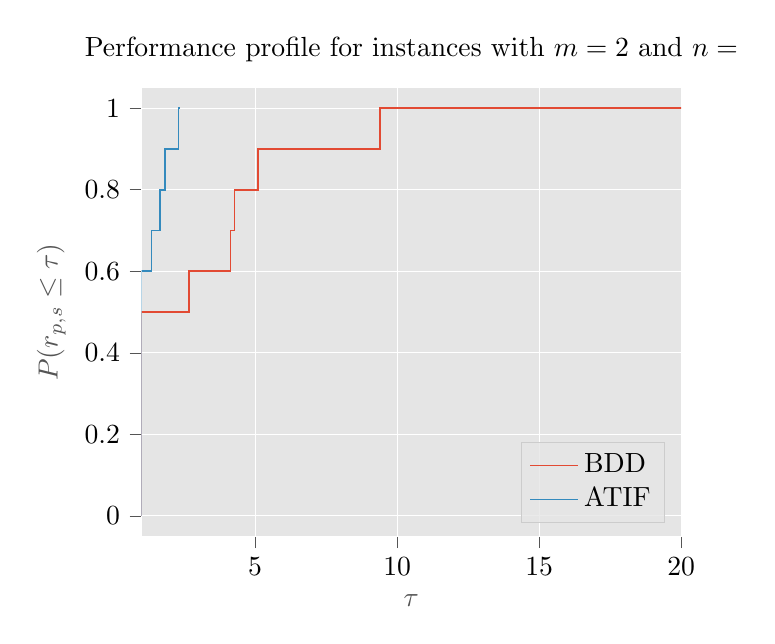
\begin{tikzpicture}

\definecolor{chocolate2267451}{RGB}{226,74,51}
\definecolor{dimgray85}{RGB}{85,85,85}
\definecolor{gainsboro229}{RGB}{229,229,229}
\definecolor{lightgray204}{RGB}{204,204,204}
\definecolor{steelblue52138189}{RGB}{52,138,189}

\begin{axis}[
axis background/.style={fill=gainsboro229},
axis line style={white},
legend cell align={left},
legend style={
  fill opacity=0.8,
  draw opacity=1,
  text opacity=1,
  at={(0.97,0.03)},
  anchor=south east,
  draw=lightgray204,
  fill=gainsboro229
},
tick align=outside,
tick pos=left,
title={Performance profile for instances with \(\displaystyle m = 2\) and \(\displaystyle n = \)},
x grid style={white},
xlabel=\textcolor{dimgray85}{\(\displaystyle \tau\)},
xmajorgrids,
xmin=1, xmax=20,
xtick style={color=dimgray85},
y grid style={white},
ylabel=\textcolor{dimgray85}{\(\displaystyle P(r_{p,s} \leq \tau)\)},
ymajorgrids,
ymin=-0.05, ymax=1.05,
ytick style={color=dimgray85}
]
\addplot [semithick, chocolate2267451, const plot mark right]
table {%
1 0
1 0.1
1 0.2
1 0.3
1 0.4
2.67356065277778 0.5
4.13041461104718 0.6
4.27739326636682 0.7
5.09894415899582 0.8
9.39336290333717 0.9
20.4255534130308 1
};
\addlegendentry{BDD}
\addplot [semithick, steelblue52138189, const plot mark right]
table {%
1 0
1 0.1
1 0.2
1 0.3
1 0.4
1 0.5
1.35734098525158 0.6
1.66099216594353 0.7
1.82994590465409 0.8
2.30255886467334 0.9
2.36687267167001 1
};
\addlegendentry{ATIF}
\end{axis}

\end{tikzpicture}
